\documentclass{pracamgr}

\usepackage{polski}
\usepackage[utf8]{inputenc}
\usepackage[pdftex]{graphicx}

\usepackage{subfig} % Subfigures
\usepackage{color}
\usepackage{ntheorem} % Definitions
\usepackage{sidecap} % Side captions to figures
\usepackage{multicol}
\usepackage{listings}
\usepackage{rotating} % Sideway figures
\usepackage{array} % Same formatting for column tables
\usepackage{multirow} % Row and columns spans
\usepackage[obeyspaces, spaces]{url} %Proper line breaking for typewriter-style texts
\usepackage{caption} %Legends with \caption*

\author{Maciej Pazurkiewicz}
\nralbumu{248267}

\title{Modelowanie sygnalizacji świetlnej}

\tytulang{Modelling of a~traffic lights system}
\kierunek{Informatyka}

\opiekun{dra hab. Sławomira Lasoty\\
  Instytut Informatyki
  }
% miesiąc i~rok:
\date{Wrzesień 2011}

%Podać dziedzinę wg klasyfikacji Socrates-Erasmus:
\dziedzina{
11.3 Informatyka\\
}

%Klasyfikacja tematyczna według AMS (matematyka) lub ACM (informatyka)
\klasyfikacja{D. Software\\
  D.2. Software engineering\\
  D.2.4. Software/Program verification}

% Słowa kluczowe:
\keywords{sygnalizacja świetlna, systemy czasu rzeczywistego, automaty
czasowe, Uppaal}

%--------------------------------------------------------------------------
% My macros
%--------------------------------------------------------------------------
\newcommand{\ang}[1]{(ang.~\emph{#1})}
\newcommand{\imgr}[1]{rys.~\ref{#1}}
\newcommand{\todo}[1]{\textcolor{red}{#1}}
\newcommand{\todocite}{\todo{[source]}}
\newcommand{\upp}{\textsc{Uppaal}}
\newcommand{\rarr}{$\rightarrow$}

%Math mode
\newcommand{\pair}[2]{\langle #1, #2 \rangle}

\theoremstyle{plain}
\theoremsymbol{\ensuremath{\clubsuit}}
\theoremseparator{.}
\theoremprework{\bigskip\begin{samepage}}
\theorempostwork{\bigskip\end{samepage}}
\newtheorem{definition}{Definicja}

%Listings
\lstdefinelanguage{Signals} {}

\lstset{
  basicstyle=\tt, extendedchars = true,
  keywordstyle=\underbar,
  emphstyle=\bf,
  %columns=fullflexible,
  xleftmargin=1cm,
  captionpos=b, abovecaptionskip=12pt, belowcaptionskip=12pt,
  delim=**[is][\ttfamily]{|}{|},
  mathescape=true,
  belowskip=.5cm,
  aboveskip=.5cm,
  language=Signals,
}
\definecolor{light-gray}{gray}{0.40}
\newcommand{\com}[1]{\upshape\color{light-gray}{#1}}

%--------------------------------------------------------------------------

\begin{document}
\maketitle

\begin{abstract}
  \todo{Napisać streszczenie.}
\end{abstract}

\tableofcontents

\chapter*{Wprowadzenie} \addcontentsline{toc}{chapter}{Wprowadzenie}

\chapter{Sygnalizacja świetlna}
\label{c:sygnalizacja}

Niniejszy rozdział zawiera informacje o~systemach sygnalizacji
świetlnej niezbędne w~dalszej części pracy. Podrozdział
\ref{s:sygn-wprowadzenie} jest wprowadzeniem do tematyki sygnalizacji,
natomiast podrozdział \ref{s:sygn-szczegoly} szczegółowo omawia
funkcjonowanie sygnalizacji wzbudzanej, będącej bazowym modelem
przedstawianego języka.

Niniejszy rozdział jest oparty na raportach przygotowanych na zlecenie
amerykańskiej agencji \emph{Federal Highway Administration}
\cite{fhwa:handbook06} \cite{fhwa:timing08}.

\section{Wprowadzenie}
\label{s:sygn-wprowadzenie}

Sygnalizacją świetlną nazywamy zestaw urządzeń przekazujących
komunikaty, służące do segregacji czasowej kolidujących potoków
ruchu. Stosuje się ją najpowszechniej na skrzyżowaniach i~przejściach
dla pieszych, lecz wykorzystywana jest także w~miejscach takich jak
przejazdy kolejowe, drogi o~ruchu wahadłowym lub drogi o~pasach
o~zmiennym kierunku ruchu.

Poprawnie zaprojektowana sygnalizacja świetlna powinna zmniejszać
prawdopodobieństwo wypadków i~kolizji oraz zapewniać odpowiedni poziom
dostępności dla pieszych i~pojazdów nadjeżdżających z~kierunków
podporządkowanych. Jednocześnie powinna zachowywać jak najwyższą
wydajność skrzyżowania rozumianą jako wysoką przepustowość, krótki
czas oczekiwania na sygnał zielony oraz małą liczbę
zatrzymań. Zapewnienie równowagi pomiędzy bezpieczeństwem a~wydajnością
należy do kluczowych elementów projektu sygnalizacji.

\subsection{Elementy systemu sygnalizacji świetlnej}
\label{ss:elementy} Najprostszy system sygnalizacji składa się
z~sygnalizatora oraz kontrolera, czyli układu logicznego decydującego
o~wyświetlanym sygnale. Współczesne systemy są często o~wiele bardziej
skomplikowane i~mogą zawierać komponenty takie jak:
\begin{description}
  \item[czujniki] -- urządzenia, które zbierają informację o~aktualnym
  zapotrzebowaniu różnych uczestników ruchu na prawo przejazdu bądź
  przejścia; są to np.~pętle indukcyjne w~jezdni bądź
  przyciski dla pieszych;
  \item[kontroler lokalny] -- urządzenie zarządzające pracą grupy
  ściśle powiązanych sygnalizatorów, np.~sterujących ruchem na jednym
  skrzyżowaniu;
  \item[kontroler główny] -- urządzenie zarządzające pracą grupy
  kontrolerów lokalnych; może być odpowiedzialny np.~za synchronizację
  sygnalizacji na ciągu skrzyżowań.
\end{description}

\subsection{Tryby pracy}
\label{ss:tryby} Sygnalizacja świetlna na skrzyżowaniach pracuje
przeważnie w~trybie stałoczasowym, wzbudzanym lub kombinacji obydwu.

\paragraph{Sygnalizacja stałoczasowa} W~systemach stałoczasowych każdy
z~potoków ruchu obsługiwany jest zgodnie ze zdefiniowanym
harmonogramem, w~którym określona jest długość każdego z~wyświetlanych
sygnałów. Akomodacja może polegać co najwyżej na zmianie harmonogramu
w~zależności od pory dnia.

\paragraph{Sygnalizacja wzbudzana}
W~trybie wzbudzanym kontroler korzysta z~informacji dostarczanych
przez czujniki, dzięki czemu może dostosować parametry pracy
sygnalizacji do aktualnych warunków ruchu. W~zależności od tego czy
czujniki są zainstalowane dla wszystkich potoków czy tylko dla
niektórych mówimy o~sygnalizacji \emph{w pełni wzbudzanej}
\ang{fully-actuated} lub \emph{częściowo wzbudzanej}
\ang{semi-actuated}.

W~systemach w~pełni wzbudzanych sygnalizacja dla każdego z~uczestników
ruchu uzależniona jest od danych dostarczonych przez czujnik.
W~szczególności oznacza to, że w~danym cyklu sygnał zielony otrzymują
tylko te fazy, na które jest zapotrzebowanie. Także czas trwania
poszczególnych sygnałów może być uzależniony od danych z~czujnika.

W~systemach częściowo wzbudzanych detekcja ruchu dotyczy tylko
niektórych potoków ruchu, np.~pieszych bądź pojazdów nadjeżdżających
z~drogi podrzędnej. Prawo przejazdu jest domyślnie przyznawane
kierunkowi głównemu; pozostałe zaś mogą je otrzymać w~wyniku
zapotrzebowania zgłoszonego przez czujnik.

\section{Sygnalizacja wzbudzana}
\label{s:sygn-szczegoly}

Niniejszy podrozdział zawiera szczegółową charakterystykę
funkcjonowania sygnalizacji wzbudzanej. Najpierw definiowane są
podstawowe pojęcia potrzebne do precyzyjnej jego specyfikacji,
następnie zaś przedstawiony jest hierarchiczny opis systemu: od
omówienia pracy pojedynczego sygnalizatora po omówienie pracy całości
sygnalizacji na skrzyżowaniu.

\subsection{Podstawowe pojęcia}
\label{ss:pojecia}

Poniżej znajdują się pojęcia, których zdefiniowanie pozwoli na
uporządkowanie i~zhierarchizowanie opisu systemu sygnalizacji
świetlnej.
\begin{description}
  \item[interwał] -- odcinek czasu, w~którym wskazanie danego
  sygnalizatora nie zmienia się; w~zależności od tego wskazania mówimy
o~  \emph{interwale zielonym}, \emph{interwale żółtym} itp.
  \item[potok ruchu] -- pojazdy bądź piesi, których ruch kontrolowany
  jest przez jeden sygnalizator\footnote{Zauważmy, że pojazdy jadące
    przez skrzyżowanie prosto oraz skręcające mogą stanowić jeden,
    dwa, a~nawet trzy oddzielne potoki w~zależności od architektury
    skrzyżowania oraz samego systemu sygnalizacji.};
  \item[faza] -- grupa potoków ruchu, którym sygnalizacja zezwala na
  jednoczesne korzystanie ze skrzyżowania;
  \item[cykl] -- ustalony ciąg faz.
\end{description}

Sygnalizator dla pojazdów wyświetla jeden z~następujących sygnałów:
czerwony, czerwono-żółty, zielony lub żółty. W~sygnalizacji dla
pieszych opuszcza się sygnał czerwono-żółty, a~żółty zastępuje się
migającym zielonym. Opis systemu sprowadza się do pokazania sposobu
wyznaczania długości interwałów odpowiadających tym sygnałom. Należy
tu uczynić dodatkową uwagę dotyczącą interwału czerwonego. Choć
w~zasadzie jego długość dla danego sygnalizatora wyznaczana jest przez
długość cyklu pracy pozostałych, to w~celu zapewnienia bezpieczeństwa
ruchu wyznacza się minimalny odcinek czasu pomiędzy zakończeniem
sygnału żółtego dla danego potoku a~rozpoczęciem sygnału
czerwono-żółtego dla potoku kolidującego. Nazywa się go okresem
oczyszczenia \ang{clearance time, all-red time} i~wyróżnia jako
dodatkowy interwał.

Sygnały czerwono-żółty, żółty, migający zielony oraz
czerwony-czyszczący nazywamy \emph{przejściowymi}. Potoki, których
sygnalizatory wyświetlają sygnał zielony lub jeden z~przejściowych,
nazywamy \emph{aktywnymi}, pozostałe zaś
\emph{nieaktywnymi}. Analogicznie, fazę, której przynajmniej jeden
potok jest aktywny nazywamy aktywną. W~danym momencie aktywna może być
co najwyżej jedna faza.

\subsection{Detekcja ruchu}
\label{ss:detekcja} Mając na celu opis systemów wzbudzanych,
rozszerzamy zestaw definicji z~\ref{ss:pojecia} o~następujące
pojęcia:
\begin{description}
  \item[zgłoszenie] -- informacja o~zapotrzebowaniu na uruchomienie
bądź przedłużenie sygnału zielonego przekazywana odpowiedniemu
kontrolerowi przez czujnik
  \item[zgłoszenie przeciwne] -- zgłoszenie pochodzące od nieaktywnego
potoku
\end{description}

\paragraph{Czujniki dla pojazdów} Czujniki wykrywające pojazdy mogą
pracować w~jednym z~dwóch trybów: \emph{pulsacyjnym} bądź
\emph{obecności}.  W~trybie pulsacyjnym \ang{pulse mode} czujnik jest
wzbudzany tylko w~momencie pojawienia się pojazdu w~zasięgu jego
działania.  Natomiast w~trybie obecności \ang{presence mode} czujnik
pozostaje wzbudzony przez cały czas od pojawienia się pojazdu
w~strefie detekcji aż do jej opuszczenia. Zgłoszenie ma zatem postać
sygnału punktowego w~przypadku trybu pulsacyjnego oraz ciągłego dla
trybu obecności.

\paragraph{Czujniki dla pieszych} Pieszy uruchamia czujnik, który
przekazuje sygnał kontrolerowi. Po zakończeniu obsługi potoku dla
pieszych kontroler przesyła informację zwrotną do czujnika, który jest
wtedy resetowany i~staje się gotowy na ponowne uruchomienie.

\subsection{Opis funkcjonowania sygnalizacji na poziomie pojedynczego
potoku}
\label{ss:schemat}

\paragraph{Cele} Bazowy schemat działania sygnalizacji wzbudzanej
powinien spełniać trzy podstawowe warunki:
\begin{enumerate}
  \item sygnał zielony jest przyznawany tylko, gdy wcześniej wykryto
oczekujące nań pojazdy;
  \item długość sygnału zielonego powinna być uzależniona od natężenia
ruchu w~danym potoku;
  \item długość oczekiwania na sygnał zielony powinna być z~góry
ograniczona.
\end{enumerate}

\paragraph{Schemat działania} W~celu realizacji powyższych założeń,
interwał zielony dzielimy na dwie części: \emph{początkową} oraz
\emph{rozszerzalną}. Długość części początkowej jest stała i~określana
przez parametr \emph{minimalny zielony}. Powinien on wynosić co
najmniej tyle, aby pozwalać na bezpieczne opuszczenie skrzyżowania
wszystkim pojazdom znajdującym się między czujnikiem a~linią
zatrzymania.

Długość części rozszerzalnej zależy od natężenia ruchu. W~momencie
otrzymania zgłoszenia sygnał zielony przedłużany jest o~tyle, aby
przejeżdżający pojazd mógł bezpiecznie opuścić skrzyżowanie (o
długości tego czasu tym decyduje inny parametr --
\emph{wydłużenie}). Gdy w~tym czasie kontroler nie otrzyma kolejnego
zgłoszenia tj. wykryta zostanie luka pomiędzy nadjeżdżającymi
pojazdami, sygnał zielony zostaje przerwany (patrz
\imgr{img:gap-out}).

\begin{figure}[h] \centering
  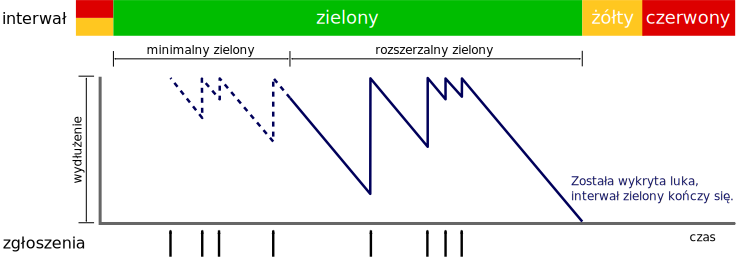
\includegraphics[width=0.7\textwidth]{img/signals-gap-out}
  \caption{Zakończenie sygnału zielonego przez wykrycie luki.}
\label{img:gap-out}
\end{figure}

Duże natężenie ruchu w~danym potoku mogłoby powodować brak luk między
pojazdami i~-- co za tym idzie~-- zbyt duże opóźnienia w~obsłudze
pozostałych potoków. Aby ograniczyć z~góry czas oczekiwania, określa
się maksymalny czas, w~którym potok może otrzymywać sygnał zielony
w~obecności zgłoszenia przeciwnego (patrz \imgr{img:max-out}). Należy
podkreślić, że w~razie braku zgłoszenia przeciwnego sygnał zielony
będzie nadawany tak długo aż nie nastąpi wykrycie luki.
\begin{figure}[h] \centering
  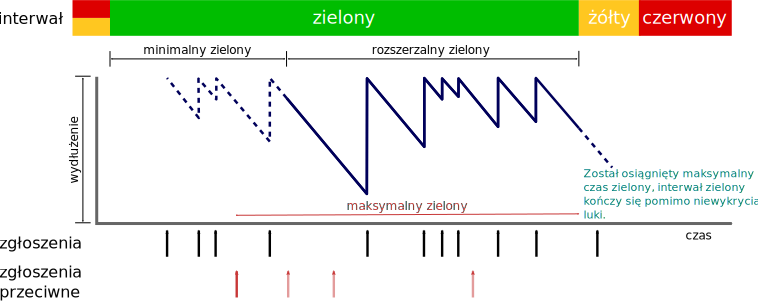
\includegraphics[width=0.7\textwidth]{img/signals-max-out}
  \caption{Zakończenie sygnału zielonego przez wykorzystanie
maksymalnego czasu.}
\label{img:max-out}
\end{figure}

\paragraph{Potoki pieszych} Tak jak w~przypadku pojazdów potok pieszy
otrzymuje sygnał zielony tylko w~wyniku zgłoszonego
zapotrzebowania. Jednak jako, że ilościowa ocena poziomu
zapotrzebowania w~przypadku ruchu pieszych jest trudna technicznie,
przyjmujemy stałą długość interwału zielonego.

\subsection{Opis funkcjonowania sygnalizacji na poziomie pojedynczej
fazy}

Podstawowym elementem opisu fazy jest stwierdzenie, które potoki
wchodzą w~jej skład. Faza może obejmować:
\begin{samepage}
\begin{itemize}
  \item jeden lub więcej potoków pojazdów,
  \item jeden lub więcej potoków pieszych,
  \item kombinację pewnej liczby potoków pojazdów i~pieszych.
\end{itemize}
\end{samepage}
\begin{figure}[h] \centering \subfloat[Faza wyłącznie dla pojazdów]{
    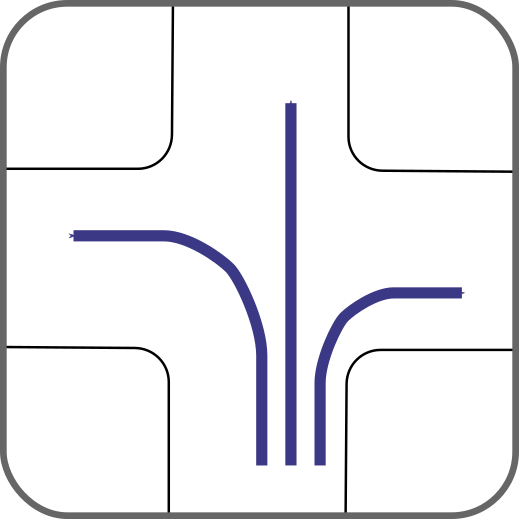
\includegraphics[width=0.27\textwidth]{img/signals-phase-example-1}
} \hfill \subfloat[Faza dla pojazdów oraz pieszych]{
    \includegraphics[width=0.27\textwidth]{img/signals-phase-example-2}
} \hfill \subfloat[Faza wyłącznie dla pieszych \ang{pedestrian
scramble, X~crossing}]{
    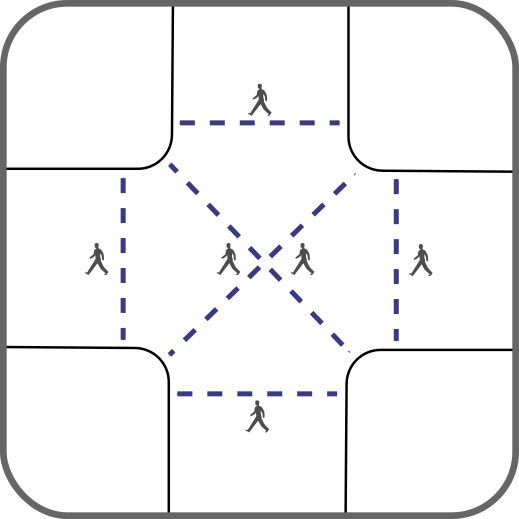
\includegraphics[width=0.27\textwidth]{img/signals-phase-example-3}
}
  \caption{Przykładowe fazy.}
\end{figure}

Zauważmy, że choć już w~opisie na poziomie potoku zaszła konieczność
zdefiniowania czasu maksymalnego, to powinien być on uważany za
właściwość fazy. Ustalenie różnych czasów maksymalnych dla różnych
potoków obniżałoby jedynie wydajność skrzyżowania w~nieuzasadniony
sposób.

Dla faz jednopotokowych nie ma potrzeby podejmowania na tym etapie
żadnych dodatkowych decyzji projektowych, gdyż opis funkcjonowania
takiej fazy jest tożsamy z~opisem funkcjonowania jej jedynego
potoku. Charakterystyka faz składających się z~wielu potoków może być
bardziej złożona, jako że dopuszczają one większą liczbę możliwych
scenariuszy. Dotyczą one sytuacji, w~których okres aktywności jednego
z~potoków mógłby być różny od okresu aktywności fazy.

\paragraph{Zgłoszenia późne} Zgłoszeniami późnymi nazywany zgłoszenia
od zgłoszenia od potoków nieaktywnych, które otrzymano już po tym, gdy
faza stała się aktywna. Po pierwsze można uznać, że zostaną obsłużone
dopiero w~następnym cyklu sygnalizacji (w takim wypadku traktowane są
tak samo jak zgłoszenia przeciwne). Drugą możliwością jest
obsługiwanie takich zgłoszeń w~bieżącym cyklu, o~ile nie spowoduje to
przekroczenia maksymalnej długości sygnału zielonego.
\begin{figure}
  \centering
  \subfloat[Opcja podtrzymania dla potoku 1 wyłączona.]{
    \includegraphics[width=0.8\textwidth]{img/signals-hold-1}
    \label{img:signals-hold-off}
  }\\\vspace{0.5cm}
  \subfloat[Opcja podtrzymania dla potoku 1 włączona.]{
    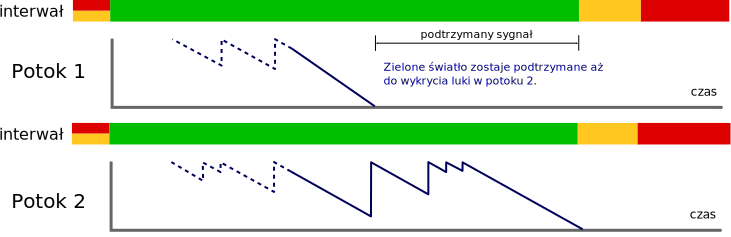
\includegraphics[width=0.8\textwidth]{img/signals-hold-2}
    \label{img:signals-hold-on}
  }
  \caption{Opcja podtrzymania sygnału dla fazy dwupotokowej.}
\end{figure}
\paragraph{Podtrzymanie} Innym elementem projektu wielopotokowej fazy
jest ustalenie zachowania się systemu w~przypadku, gdy w~jednym
z~aktywnych potoków wykryta została luka, w~innym zaś mamy do czynienia
z~ciągłym zapotrzebowaniem. Możemy nie podejmować żadnego specjalnego
działania tj. wyłączyć sygnał zielony dla potoku, w~którym czujnik
wykrył lukę (rys. \ref{img:signals-hold-off}).  Można w~takim przypadku
zastosować także procedurę \emph{podtrzymania sygnału} \ang{hold}. Polega
ona na wydłużeniu sygnału aż do momentu, w~którym zakończą się sygnały
zielone dla pozostałych potoków (rys. \ref{img:signals-hold-on}).

\subsection{Opis funkcjonowania sygnalizacji na poziomie cyklu}
Opis cyklu zawiera przede wszystkim informację o~kolejności
wchodzących w~jego skład faz.
\begin{figure} \centering
  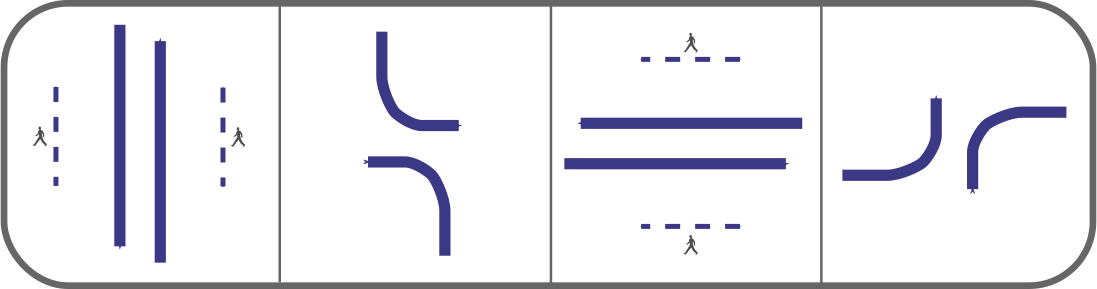
\includegraphics[width=0.7\textwidth]{img/signals-cycle-example}
  \caption{Przykładowy cykl.}
\end{figure}
Jedyną dodatkową decyzją pozostającą do podjęcia na tym etapie jest
zachowanie się sygnalizacji w~przypadku braku zgłoszeń tj.
w~\emph{stanie spoczynku} \ang{rest}. Stosowane są dwa rozwiązania. Po
pierwsze wszystkie sygnalizatory mogą wyświetlać sygnał czerwony
\ang{rest in red}. Po drugie można wybrać fazę domyślną, która będzie
aktywna w~przypadku braku jakiegokolwiek zapotrzebowania.

\subsection{Podsumowanie}

W~rozdziale zaprezentowany został kompozycjonalny sposób opisu
systemów sygnalizacji wzbudzanej. Na początku zdefiniowano zachowanie
się sygnalizacji dla pojedynczego potoku, następnie potoki zostały
złożone w~fazy, a~fazy -- w~cykl. Na każdym etapach dokładamy
informacje specyfikujące sposób owego złożenia.

Poniższe zestawienie podsumowuje parametry zawarte w~poszczególnych
warstwach opisu.
\begin{enumerate}
  \item \textbf{Potok ruchu:}
  \begin{itemize}
    \item typ potoku: dla pojazdów / dla pieszych,
    \item tryb pracy i rozmieszczenie czujników,
    \item długości interwałów przejściowych:
    \begin{itemize}
      \item czerwono-żółty,
      \item żółty,
      \item okres czyszczenia;
    \end{itemize}
    \item parametry decydujące o~długości interwału zielonego:
    \begin{itemize}
      \item minimalny zielony,
      \item wydłużenie;
    \end{itemize}
  \end{itemize}
  \item \textbf{Faza:}
  \begin{itemize}
    \item potoki składające się na fazę,
    \item maksymalny zielony,
    \item obsługa późnych zgłoszeń,
    \item podtrzymanie sygnału zielonego;
  \end{itemize}
  \item \textbf{Cykl:}
  \begin{itemize}
    \item fazy wchodzące w~skład cyklu i~ich kolejność,
    \item zachowanie w~stanie spoczynku.
  \end{itemize}
\end{enumerate}

\chapter{Automaty czasowe}
\label{c:ta}
Automaty czasowe są teoretycznym narzędziem umożliwiającym modelowanie
i~weryfikację systemów czasu rzeczywistego. Po zdefiniowaniu ich przez
Alura i~Dilla \cite{alur-dill} nie tylko stały się popularnym obszarem
badań teoretyków, lecz były także stosowane w~praktycznych problemach
weryfikacyjnych.

Podrozdział \ref{ta-theory} wprowadza definicję automatów czasowych
oraz zawiera najważniejsze informacje z~teorii z~nimi związanej;
natomiast \ref{uppaal} opisuje \upp-a -- zastosowane w~pracy narzędzie
do weryfikacji systemów modelowanych przy pomocy automatów czasowych.

\section{Automaty czasowe}
\label{ta-theory}

Wersja formalizmu automatów czasowych przedstawiona w~niniejszym
rozdziale pochodzi od Henzingera i~in.\cite{henz-94}. Jej teoretyczna
siła wyrazu jest identyczna z~siłą wyrazu automatów w~wersji Alura
i~Dilla, natomiast jest ona wygodniejsza do praktycznego modelowania
systemów.

Automat czasowy jest zwykłym automatem skończonym rozszerzonym
o~zestaw zmiennych rzeczywistych nazywanych zegarami. Stanem takie
automatu będziemy nazywali parę składającą się z:
\begin{itemize}
  \item wierzchołka (tj. stanu odpowiedniego automatu skończonego),
  \item wartościowania zegarów.
\end{itemize}
W~stanie początkowym wartości wszystkich zegarów są wyzerowane,
natomiast w~czasie jego działania wszystkie zwiększają swoją wartość
w~tym samym tempie. Przyrost wartości zegarów modeluje upływ czasu.

Aby móc modelować systemy o~pożądanych własnościach, możemy nakładać
pewne dodatkowe warunki na tranzycje oraz wierzchołki. Każdej
tranzycji możemy przypisać wyrażenie opisujące wartościowanie zegarów,
przy którym jej wykonanie jest dozwolone. Analogiczne ograniczenia dla
wierzchołków nazywane są \emph{niezmiennikami}. Poprawne są tylko te
stany automatu czasowego, w~których wartościowanie zegarów spełnia
niezmiennik danego wierzchołka. Jedyną dozwoloną operacją na zegarze
jest jego resetowanie, czyli ustawienie jego wartości na
zero. Przykładowy automat przedstawiono na \imgr{img:ta-simple}.

\begin{SCfigure}[4]
  \centering
  \includegraphics[width=0.3\textwidth]{img/ta-simple}
  \caption {Przykładowy automat czasowy z~jednym zegarem~$t$.
    Czcionką zieloną oznaczone są ograniczenia na krawędzie, fioletową
    niezmienniki wierzchołków, zaś niebieską -- operacje resetowania
    zegara.\\ Automat zaczyna pracę w~wierzchołku czerwonym, w~którym
    przebywa dokładnie przez 10 jednostek czasu. Następnie przechodzi
    do wierzchołka zielonego (5-10 jednostek, niedeterministycznie)
i~    pomarańczowego (dokładnie 3~jednostki), po czym powraca do stanu
    początkowego.}
  \label{img:ta-simple}
\end{SCfigure}

\subsection{Formalna definicja} Przyjmijmy, że mamy skończony zbiór
$\mathcal{C}$ zmiennych rzeczywistych (zegarów) oraz skończony alfabet
$\Sigma$ (akcji).

\begin{definition}[Ograniczenie zegarowe] Ograniczeniem zegarowym
nazywamy koniunkcję formuł o~postaci $x \sim n$ bądź $x - y~\sim n$,
gdzie $x, y~\in \mathcal{C}$, $n \in \mathbf{N}$, natomiast $\sim$
jest jedną spośród relacji $=, \le, \leq, \ge, \geq$.
\end{definition}
Zbiór ograniczeń zegarowych nad $\mathcal{C}$ będziemy oznaczali przez
$\mathcal{B}(\mathcal{C})$.

\begin{definition}[Automat czasowy] Automat czasowy jest $\mathcal{A}$
jest krotką $\langle N, l_0, E, I\rangle$, gdzie
  \begin{itemize}
    \item $N$ jest skończonym zbiorem wierzchołków,
    \item $l_0$ jest wierzchołkiem początkowym,
    \item $E \subseteq N~\times \mathcal{B}(\mathcal{C}) \times \Sigma
    \times 2^{\mathcal{C}} \times N$ jest zbiorem krawędzi
    \item $I: N~\mapsto \mathcal{B}(\mathcal{C})$ jest funkcją
    przypisującą wierzchołkom ich niezmienniki
  \end{itemize}
\end{definition}
Zamiast $\langle l, g, a, r, l' \rangle \in E$ będziemy pisali $l
\stackrel{g, a, r}{\longrightarrow} l'$. Zapis taki oznacza tranzycję
$a$ prowadzącą z~wierzchołka $l$ do wierzchołka $l'$, którą można
wykonać przy wartościowaniu zegarów spełniającym ograniczenie $g$
i~przypisującą $0$ wszystkim zegarom z~$r$.

Tak zdefiniowany automat czasowy rozumiemy jako
system przejść, w~którym można wykonywać dwa rodzaje tranzycji:
\begin{description}
  \item[opóźnienie] polega na zwiększeniu wartości wszystkich zegarów
  o~pewną liczbę rzeczywistą; intuicyjnie, jest to przebywanie przez
  jakiś czas w~wierzchołku;
  \item[wykonanie akcji] polega na przejściu do innego wierzchołka
  zgodnie z~wybraną krawędzią; wykonanie akcji nie jest związane
  z~upływem czasu (zmiana wartościowania zegarów może wynikać jedynie
  ze zresetowania niektórych z~nich).
\end{description}
Formalnie ujmuje to poniższa definicja.
\begin{definition}[Semantyka operacyjna automatu czasowego] Semantyką
  automatu czasowego jest system przejść, którego stany są parami
  $\pair{l}{u}$ a~przejścia spełniają następujące reguły:
  \begin{itemize}
    \item $\pair{l}{u} \stackrel{d}{\longrightarrow} \pair{l}{u+d}$
    jeśli $u \vdash I(l)$ oraz $(u+d) \vdash I(l)$ dla pewnego $d \in
    \mathbf{R}^{+}$
    \item $\pair{l}{u} \stackrel{a}{\longrightarrow} \pair{l'}{u'}$,
    jeśli $l \stackrel{g, a, r}{\longrightarrow} l', u~\vdash g, u' =
    [r \mapsto 0]u$ oraz $u' \in I(l')$
  \end{itemize}
\end{definition}

\subsection{Problemy weryfikacyjne}

Liczba stanów tak zdefiniowanego automatu jest nieprzeliczalna, co
sprawia, że wydaje się, że nie są odpowiednim modelem dla zadań
weryfikacyjnych. Rozwiązanie tego problemu zaproponowali już Alur
i~Dill \cite{alur-dill}, zauważając, że pewnych własności można dowodzić,
opierając się na skończonej abstrakcji automatu.

Wprowadzona przez nich abstrakcja nazywa się \emph{równoważnością
  regionów}. Opiera się na spostrzeżeniu, że dwa stany automatu są
równoważne, gdy:
\begin{samepage}
\begin{enumerate}
  \item wartości zegarów zgadzają się co do części całkowitej,
  \item zachowany jest porządek na częściach ułamkowych zegarów.
\end{enumerate}
\end{samepage}
Intuicyjnie, pierwsza własność odpowiada za sprawdzenie czy spełnione
jest dane ograniczenie zegarowe; natomiast dzięki drugiej wiadomo,
wartość którego zegara przekroczy jako pierwsza kolejną liczbę
naturalną \cite{am:decision}. Po dodatkowym utożsamieniu ze sobą stanów,
w~których wartości zegarów są większe niż odpowiednie maksymalne stałe
z~ograniczeń, zyskujemy skończoną abstrakcję dla wartościowań zegarów
(rys. \ref{img:regions}).
\begin{figure}
  \centering
  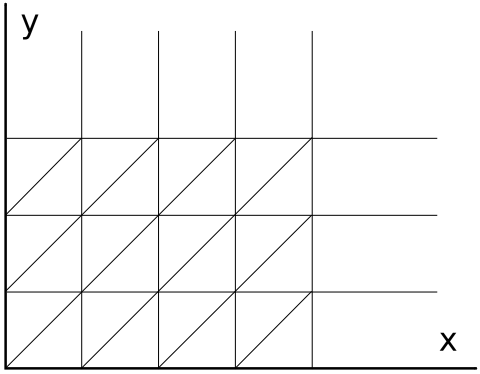
\includegraphics[width=0.4\textwidth]{img/ta-regions}
  \caption{Regiony dla automatu o~dwóch zegarach (każdy punkt
    przecięcia, odcinek, półprosta oraz ograniczony nimi fragment
    płaszczyzny reprezentują oddzielny region). \todo{Poprawić (albo
      zmienić definicję)!}}
  \label{img:regions}
\end{figure}

Opierając się na równoważności regionów, można skonstruować
\emph{automat regionów}, w~którym stany są parami $\pair{l}{r}$, gdzie
$l$ jest wierzchołkiem wyjściowego automatu, zaś $r$ pewnym
regionem. Jest to automat skończony, zatem można dla niego efektywnie
rozstrzygać np.~problem osiągalności wierzchołka bądź pustości języka.

Chociaż równoważność regionów jest bardzo wygodnym pojęciem
w~teoretycznych badaniach własności automatów czasowych, nie stosuje się
go w~rzeczywistych problemach weryfikacyjnych. Rozmiar automatu
regionów jest bowiem wykładniczy ze względu na liczbę zegarów oraz
górne ograniczenia ich wartości.

Bardziej zgrubnej -- niemniej wystarczająco dokładnej dla
weryfikacji-- abstrakcji automatu czasowego dokonuje się przy pomocy
\emph{stref} \cite{henz-94}. Strefą nazywamy maksymalny zbiór
wartościowań zegarów spełniających koniunkcję ograniczeń zegarowych.
Rysunek \ref{img:zones} przedstawia automat czasowy i~odpowiadający mu
automat stref.

\begin{figure}
  \centering
  \subfloat[Przykładowy automat czasowy.] {
    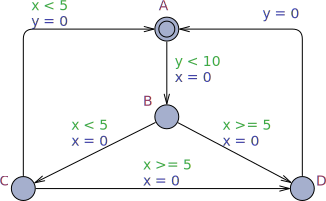
\includegraphics[width=0.35\textwidth]{img/ta-zones-example-1}
  } \hspace{1cm}
  \subfloat[Odpowiadający mu automat stref.] {
    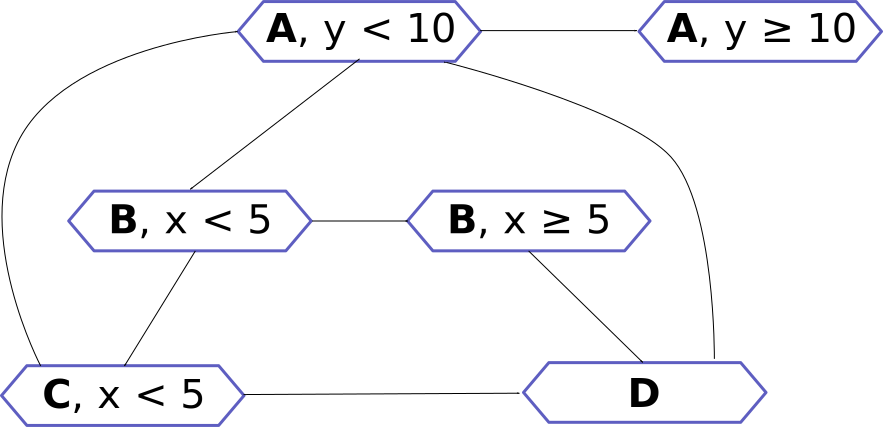
\includegraphics[width=0.35\textwidth]{img/ta-zones}
  }
  \caption{Strefy.}
  \label{img:zones}
\end{figure}

\section{\upp}
\label{uppaal}

\upp\ jest zestawem narzędzi pozwalającym na modelowanie systemów czasu
rzeczywistego przy pomocy automatów czasowych, ich symulację a~także
weryfikację ich własności. Rozwijają go wspólnie Uniwersytet w~Uppsali
oraz Uniwersytet w~Aalborg. Pierwsza wersja narzędzia została wydana w~roku
1995 \cite{lpw:fct95}.

\upp\ był wielokrotnie wykorzystywany w~weryfikacji rzeczywistych
systemów: od protokołów komunikacyjnych po aplikacje multimedialne
(m.in. \cite{lp:prfts97}, \cite{lpw:tacas98},
\cite{DBLP:conf/icfem/BordbarO03},
\cite{Ravn:2011:MVW:1987389.1987431}). Był jednym z~głównym narzędzi
stosowanych w~-- prowadzonym przez konsorcjum europejskich
uniwersytetów i~przedsiębiorstw -- projekcie \textsc{Ametist}, mającym
na celu rozwój efektywnych metod weryfikacji przemysłowych systemów czasu
rzeczywistego \cite{AMETISTfinal}.

\subsection{Modelowanie}
Modelowanie w~\upp-u polega nie tyle na tworzeniu jednego automatu
czasowego, lecz projektowaniu \emph{szablonów} automatów, których
instancje -- nazywane procesami -- tworzą model całego systemu. Dzięki
temu model podzielić na logiczne części o~ściśle określonych
odpowiedzialnościach.

Model projektuje się przy pomocy prostego graficznego interfejsu
użytkownika (patrz rys.~\ref{img:uppaal-gui}). Wbudowany w~aplikację
symulator pozwala na szybkie zapoznanie się z~funkcjonowaniem modelu,
a~także ułatwia przeglądanie kontrprzykładów dostarczanych przez
weryfikator. Co ważne, symulator pokazuje nie konkretne stany systemu,
a~stany symboliczne (strefy). Przydatną funkcją jest także generacja
diagramu komunikacji procesów trakcie symulacji
(rys.~\ref{img:uppaal-msc}).
\begin{figure}
  \centering
  \includegraphics[width=0.9\textwidth]{img/uppaal-editor.png}
  \caption{Interfejs edytora szablonów procesów.}
  \label{img:uppaal-gui}
\end{figure}

\begin{figure}
  \centering
  \includegraphics[width=0.8\textwidth]{img/uppaal-msc.png}
  \caption{Generowany przez symulator \upp-a diagram komunikacji
    procesów \ang{message sequence chart}.}
  \label{img:uppaal-msc}
\end{figure}

Autorzy \upp-a rozszerzyli podstawową definicję automatów czasowych
o~dodatkowe konstrukcje. Większość nie zwiększa siły
wyrazu formalizmu, a~jedynie ułatwia modelowanie bardziej złożonych
systemów.  Poniżej opisane zostaną najważniejsze rozszerzenia
(ich wyczerpujący opis wraz z~formalnie zdefiniowaną semantyką
odnaleźć można w~\cite{by-lncs04}).
\paragraph{Procesy i~ich komunikacja} Możliwość modelowania przy
pomocy sieci automatów czasowych wiąże się z~koniecznością
wprowadzenia mechanizmu komunikacji pomiędzy poszczególnymi
procesami. W~\upp-u jest ona realizowana poprzez synchronizację na
kanałach komunikacyjnych. Dwa procesy synchronizują się na kanale
komunikacyjnym \texttt{a}, gdy jeden z~nich wykonuje z~nich
akcję~\texttt{a?}, a~drugi --~\texttt{a!}. Kanał komunikacyjny może
być zadeklarowany także jako \emph{rozgłoszeniowy} \ang{broadcast}, co
pozwala na synchronizację \emph{jeden do wielu}.
\begin{SCfigure}[3]
  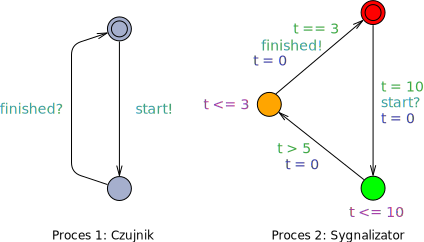
\includegraphics[width=0.6\textwidth]{img/ta-communication}
  \caption[Synchronizujące się ze sobą automaty czasowe.]
  {Synchronizujące się ze sobą automaty czasowe. System składa się
z~    dwóch procesów: czujnika i~sygnalizatora. Proces sygnalizatora
    przypomina ten z~\imgr{img:ta-simple}; w~tym wypadku jednak czas
    przebywania w~wierzchołku czerwonym nie jest stały, lecz
    wyznaczany przez proces czujnika. Czujnik wysyła polecenie
    początku pracy \texttt{start!}, a~następnie czeka na informację
o~    jej zakończeniu na kanale \texttt{finished}.}
\end{SCfigure}

\paragraph{Zmienne całkowitoliczbowe} Obok zmiennych zegarowych
użytkownik może deklarować także zmienne całkowitoliczbowe oraz
tablice. Wyrażeń na nich można używać w~ograniczeniach na krawędziach
oraz niezmiennikach wierzchołków. Przypisania na zmienne wykonywane są
w~trakcie przejścia, analogicznie do resetowania zegarów.

\paragraph{Wierzchołki pilne oraz przymusowe} Wprowadzono możliwość
dodatkowego oznaczenia wierzchołków automatów jako \emph{pilne}
\ang{urgent} bądź \emph{przymusowe} \ang{committed}.

Jeśli automat jest w~wierzchołku pilnym, nie może wykonać opóźnienia
(żaden czas nie może upłynąć). Jest to równoważne zadeklarowaniu
dodatkowego zegara $t$, który będzie resetowany na wszystkich
krawędziach wchodzących do danego wierzchołka oraz nadaniu mu
niezmiennika $t \leq 0$ (\imgr{img:uppaal-urgent}). Jako pilne mogą być
oznaczone także kanały komunikacyjne; procesy muszą się
zsynchronizować na takim kanale tak szybko jak będzie to możliwe.

\begin{figure}[h]
  \centering
  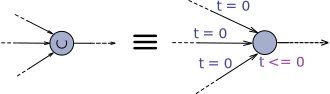
\includegraphics[width=.5\textwidth]{img/uppaal-urgent}
  \caption{Wierzchołek pilny i~równoważny mu wierzchołek z~dodatkowym
    zegarem.}
  \label{img:uppaal-urgent}
\end{figure}

Jeszcze silniejszą własność mają wierzchołki przymusowe. Są to
wierzchołki pilne, z~których przejście należy wykonać tak szybko jak
to możliwe. Jeśli któryś z~procesów jest w~wierzchołku przymusowym,
system nie może wykonać przejścia z~wierzchołka nieprzymusowego.
Wierzchołki przymusowe są bardzo przydatne np.~w~modelowaniu atomowych
ciągów komunikacji pomiędzy wieloma procesami.

\subsection{Weryfikacja}

Weryfikator \upp-a pozwala na dowodzenie własności opisywanych przez
podzbiór języka TCTL \cite{acd:mc}. Poprawne są wszystkie formuły
następujących postaci \cite{by-lncs04}:
\begin{itemize}
  \item \texttt{A[] $\varphi$} -- ,,zawsze $\varphi$'' (bezpieczeństwo),
  \item \texttt{E<> $\varphi$} -- ,,być może kiedyś $\varphi$''
  (osiągalność),
  \item \texttt{A<> $\varphi$} -- ,,zawsze kiedyś $\varphi$'',
  \item \texttt{E[] $\varphi$} -- ,,być może zawsze $\varphi$''
  \item \texttt{$\varphi$ --> $\psi$}\footnote{W czystym TCTL własność
    ta zostałaby zapisana następująco: \texttt{A[]
      ($\varphi\rightarrow$ A<> $\psi)$}} -- ,,$\varphi$ zawsze
  prowadzi do $\psi$'' (żywotność),
\end{itemize}
gdzie $\varphi$ i~$\psi$ są własnościami stanu tj. predykatami
dotyczącymi wierzchołków oraz zmiennych liczbowych i~zegarów.
Dodatkowo dostępny jest predykat \texttt{deadlock} prawdziwy
w~stanach, w~których nastąpiło zakleszczenie tj. nie można wykonać
żadnego dozwolonego przejścia.

Semantykę powyższych formuł określamy, rozwijając kolejne
przejścia w~potencjalnie nieskończone drzewo. Litery \texttt{A}
i~\texttt{E} w~formułach wprowadzają kwantyfikację po ścieżkach tego drzewa:
\texttt{A} oznacza, że dana własność ma być spełniona dla wszystkich
ścieżek, zaś \texttt{E} -- dla co najmniej jednej. Symbole
\texttt{[]} oraz \texttt{<>} kwantyfikują stany na pojedynczej
ścieżce: \texttt{[]} mówi, że własność ma być spełniona dla wszystkich
stanach na ścieżce, zaś \texttt{<>} -- w~co najmniej jednym.

\begin{figure}
  \centering
  \subfloat[{\texttt{A[] $\varphi$}}]{
    \includegraphics[width=0.3\textwidth]{img/uppaal-tctl-1}
  }
  \subfloat[\texttt{A<> $\varphi$}]{
    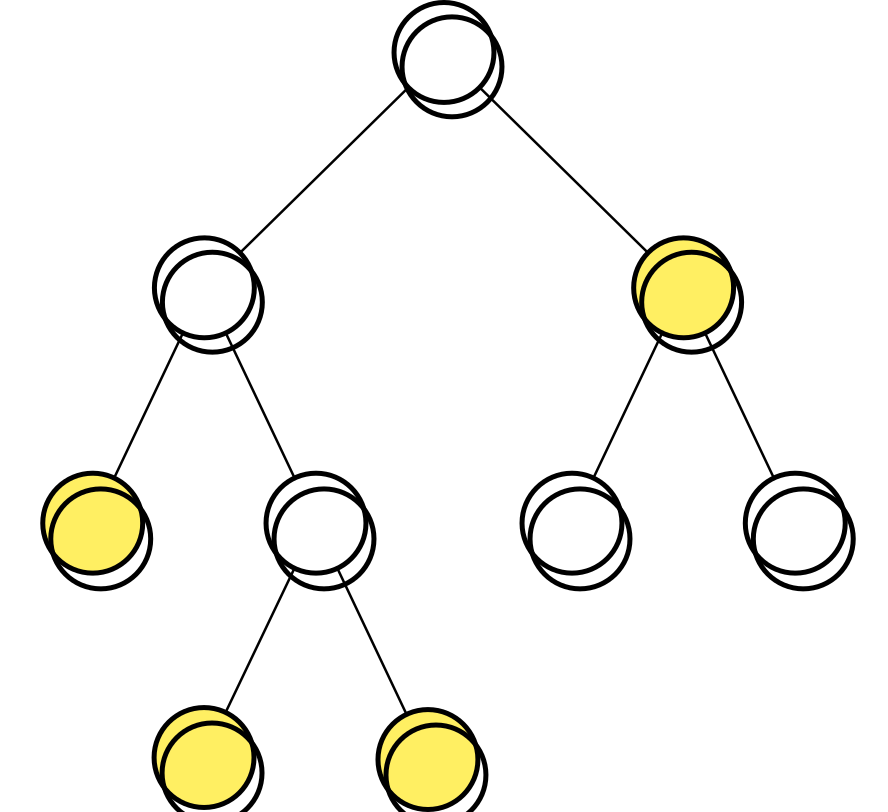
\includegraphics[width=0.3\textwidth]{img/uppaal-tctl-2}
  }\\
  \subfloat[\texttt{E[] $\varphi$}]{
    \includegraphics[width=0.3\textwidth]{img/uppaal-tctl-3}
  }
  \subfloat[\texttt{E<> $\varphi$}]{
    \includegraphics[width=0.3\textwidth]{img/uppaal-tctl-4}
  }
  \subfloat[\texttt{$\varphi$ --> $\psi$}]{
    \includegraphics[width=0.3\textwidth]{img/uppaal-tctl-5}
  }
  \caption{Własności TCTL.}
  \label{img:tctl-props}
\end{figure}

W~celu ułatwienia weryfikacji ilościowej autorzy \upp-a rozszerzyli
przedstawiony język własności o~zapytania \texttt{sup} i~\texttt{inf}.
Zapytanie \texttt{sup$\{\varphi\}$: x} daje w~wyniku największą wartość,
którą może przyjąć zmienna $x$ w~stanie spełniającym predykat $\varphi$.
Analogicznie, zapytanie \texttt{inf} podaje najmniejszą osiągalną wartość.

\chapter{Język modelowania}

Choć modelowanie systemów czasu rzeczywistego -- w szczególności
systemów sygnalizacji świetlnej -- automatami czasowymi niesie ze sobą
wiele korzyści, może być ono zadaniem skomplikowanym i
czasochłonnym. Wynika to ze swego rodzaju niskopoziomowości tego
formalizmu. Rozwiązaniem tego problemu jest wprowadzenie
sformalizowanego opisu stanowiącego warstwę pośrednią pomiędzy
rzeczywistym systemem a jego modelem w języku automatów czasowych.

Podrozdział \ref{c:lang:req} przedstawia podstawowe wymagania, które
powinien spełniać język formalnego modelowania oraz potencjalne
korzyści wynikające z jego stosowania, natomiast podrozdział
\ref{c:lang:lang} zawiera opis proponowanej składni takiego języka.

\section{Wymagania i korzyści}
\label{c:lang:req}

\subsection{Pożądane własności}

Kluczowym wymaganiem stawianym specyfikacji w prezentowanym języku
modelowania jest możliwość jej automatycznego przekształcenia w model
w języku automatów czasowych. Po pierwsze daje to jednoznaczną
semantykę takiego opisu: wątpliwości można rozstrzygnąć, symulując
działanie modelu w wybranym scenariuszu. Po drugie zaś -- udostępnia
korzyści wynikające z włączenia do projektu formalnych modeli bez
potrzeby ich ręcznego konstruowania.

Kolejnymi pożądanymi cechami omawianego języka modelowania są prostota
i wysokopoziomowość. W celu ich zapewnienia należy zawęzić dziedzinę
języka wyłącznie do systemów sygnalizacji świetlnej, dbając
jednocześnie o to, aby był on dostatecznie elastyczny, by w przyjętej
formie można było wyspecyfikować jak najliczniejszy zbiór stosowanych
rozwiązań. Aby ułatwić modelowanie, składnia języka powinna być oparta
na istniejącym aparacie pojęciowym.

\subsection{Oczekiwane korzyści}
\label{ss:lang:req:benefits}
Formalny opis w języku spełniającym powyższe wymagania powinien
stanowić realną wartość dodaną w projekcie systemu sygnalizacji
świetlnej. Przede wszystkim, byłby on usystematyzowaną
specyfikacją precyzyjnie określającą sposób jego funkcjonowania. Po
drugie automatyczna generacja modeli pozwoliłaby na szybkie i
niepodatne na błędy modyfikowanie projektu oraz ponowną weryfikację jego
własności. Formalne opisy oraz wygenerowane modele mogłyby być także
wykorzystywane jako podstawa do wprowadzania własnych rozszerzeń już
na poziomie automatów czasowych.

Zauważmy, że wprowadzenie warstwy pośredniej nie tylko ułatwiłoby
modelowanie automatami czasowymi osobom znającym ten formalizm, ale
także dałoby dostęp do korzyści wynikających z jego stosowania osobom
z nim niezaznajomionym.

% Przydaje się także do tego, że czasem chcemy dodać do modelu
% coś co jest potrzebne tylko w weryfikacji.

\section{Składnia}
\label{c:lang:lang}
Specyfikacja systemu sygnalizacji świetlnej w przedstawianym języku
składa się z opisów warstw tj. potoków, faz oraz cyklu.
Podział parametrów pomiędzy poszczególne warstwy jest zgodny
z treścią rozdziału \ref{c:sygnalizacja}.

Składnia bazuje formacie YAML\cite{YAML}. Sprawia to, że jest ona
zarówno czytelna dla człowieka jak i łatwa w przetwarzaniu
maszynowym. Opis w każdej warstwie jest po prostu słownikiem wartości
odpowiednich parametrów.


\subsection{Elementy wstępne}
Aby uprościć dalszy opis wprowadzamy następujące pomocnicze typy danych:
\lstset{
  emph={movement, id, user, length, intervals, red_amber, amber,
    red_clear, green, max_green, min_green, gap, movements, hold,
    late, flashing, max_time, phases, rest},
  emph=[2]{movement, phase, cycle},
  emphstyle=[2]\underbar,
  morecomment=[l][\color{light-gray}]{//},
  extendedchars=true,
  texcl=true,
  frame=lines
}
\begin{lstlisting}
   mvmt_id  == int[0..m]   // \com{m -- liczba potoków}
   phase_id == int[0..p]   // \com{p -- liczba faz}
   time                    // \com{długość odcinka czasu}
\end{lstlisting}

\subsection{Potok ruchu}
Na poziomie potoku definiujemy jego identyfikator, typ uczestnika
ruchu (\texttt{user}) oraz długości poszczególnych interwałów.  Dla
sygnału zielonego o zmiennej długości określamy parametry
\emph{minimalny zielony} (\texttt{min\_green}) oraz \emph{wydłużenie}
(\texttt{gap}). Jeśli jego długość jest stała wystarczy proste
określenie typu \texttt{time}\footnote{Standardowo w sygnalizacji
  wzbudzanej sygnał zielony ma zmienną długość dla pojazdów i stałą --
dla pieszych. Takie rozwiązanie przedstawiono w listingu. Oczywiście
nic nie stoi na przeszkodzie, aby potokowi pojazdów także przypisać
stałą długość sygnału zielonego.}.

\noindent\begin{minipage}{1.0\linewidth}
\begin{lstlisting}[caption=Schemat opisu potoku pojazdów.]
movement
   id:     mvmt_id
   user:   VEHICLE
   intervals:
      green:
         min_green: time
         gap:       time
      red_amber: time
      amber:     time
      red_clear: time
\end{lstlisting}
\end{minipage}

\noindent\begin{minipage}{1.0\linewidth}
\begin{lstlisting}[caption=Schemat opisu dla potoku pieszych.]
movement
   id:     mvmt_id
   user:   PEDESTRIAN
   intervals:
      green    : time
      flashing : time
      red_clear: time
\end{lstlisting}
\end{minipage}

\subsection{Faza} Specyfikacja dla fazy obejmuje przede wszystkim jej
unikalny identyfikator oraz listę składających się na nią potoków.
Gdy przynajmniej jeden z potoków należących do fazy ma zmienną długość
okresu aktywności, należy zdefiniować parametr maksymalny zielony
(\texttt{max\_time}).  Dodatkowo dla faz wielopotokowych zdefiniować
można listy potoków:
\begin{itemize}
  \item dla których stosowana będzie procedura podtrzymania sygnału
  (lista \texttt{hold});
  \item dla których zgłoszenia późne będą -- w miarę możliwości --
  obsługiwane w bieżącym okresie aktywności fazy (lista \texttt{late}).
\end{itemize}
\noindent\begin{minipage}{1.0\linewidth}
\begin{lstlisting}[caption=Schemat opisu fazy.]
phase:
   id: phase_id
   movements: list of mvmt_id
   max_time : time
   hold: list of mvmt_id
   late: list of mvmt_id
\end{lstlisting}
\end{minipage}

\subsection{Cykl} Podstawowym elementem definicji cyklu jest
uporządkowana lista faz wchodzących w jego skład. Dodatkowo określić
należy zachowanie się sygnalizacji w stanie spoczynku (parametr
\texttt{rest}). Wartością tego parametru może być identyfikator fazy,
która ma być wtedy obsługiwana, bądź stała \texttt{REST-IN-RED},
oznaczająca nadawanie sygnału czerwonego wszystkim potokom.

\noindent\begin{minipage}{1.0\linewidth}
\begin{lstlisting}[caption=Schemat opisu cyklu.]
cycle:
   phases: list of phase_id
   rest: phase_id | REST-IN-RED
\end{lstlisting}
\end{minipage}
  
\subsection{Przykład kompletnej specyfikacji}
%\noindent\begin{minipage}{1.0\linewidth}
\begin{lstlisting}[caption=Schemat opisu potoku pojazdów.]
movement
   id:     mvmt_id
   user:   VEHICLE
   intervals:
      green:
         min_green: time
         gap:       time
      red_amber: time
      amber:     time
      red_clear: time

movement
   id:     mvmt_id
   user:   VEHICLE
   intervals:
      green:
         min_green: time
         gap:       time
      red_amber: time
      amber:     time
      red_clear: time

movement
   id:     mvmt_id
   user:   VEHICLE
   intervals:
      green:
         min_green: time
         gap:       time
      red_amber: time
      amber:     time
      red_clear: time
movement
   id:     mvmt_id
   user:   VEHICLE
   intervals:
      green:
         min_green: time
         gap:       time
      red_amber: time
      amber:     time
      red_clear: time

movement
   id:     mvmt_id
   user:   PEDESTRIAN
   intervals:
      green    : time
      flashing : time
      red_clear: time
\end{lstlisting}
%\end{minipage}
\chapter{Modele}
Kluczową kwestią niezbędną dla osiągnięcia pełni korzyści wymienionych
w \ref{ss:lang:req:benefits} jest wysoka jakość generowanych
modeli. Niniejszy rozdział przedstawia najważniejsze kwestie związane z
ich konstrukcją.

Podrozdział \ref{s:models:assumptions} zawiera opis dodatkowych
założeń, które przyjęto, projektując modele. Podrozdział
\ref{s:models:models} przedstawia podział systemu na komponenty, ich
strukturę oraz podstawowy schemat działania, natomiast
\ref{s:models:project} omawia najważniejsze decyzje projektowe.

\section{Założenia}
\label{s:models:assumptions}

Przyjęcie upraszczających rzeczywistość założeń wynika z samej istoty
modelowania. Ich źródłem mogą być zarówno cechy samego systemu jak i
formalizm przyjęty jako język modelowania.

Przyjęto następujące założenia o ruchu pojazdów i pracy czujników:
\begin{itemize}
  \item Każde zgłoszenie otrzymane w trakcie interwału zielonego uważa
  się za obsłużone tj. przyjmuje się, że pojazd, od którego pochodzi,
  opuszcza skrzyżowanie. Pominięte zostają scenariusze, w których
  czujnik zostanie wzbudzony w trakcie interwału zielonego, lecz
  pojazd nie opuści skrzyżowania.
  \item Każde zgłoszenie przyjęte poza interwałem zielonym będzie
  obsłużone w przyszłości tj. w końcu zostanie wyświetlony sygnał
  zielony. Stanie się tak także wtedy, gdy właściwy pojazd opuści
  skrzyżowanie wcześniej. 
\end{itemize}
Formalnym ujęciem powyższych założeń jest następująca własność
żywotności, której spełnienia będziemy oczekiwali od stworzonych
modeli sygnalizacji: przyjęcie zgłoszenia oznacza, że albo sygnał
zielony jest właśnie wyświetlany, albo zostanie on w końcu
wyświetlony.

Źródłem następnego założenia jest formalizm automatów czasowych. Nie
nakłada on żadnych ograniczeń na czas, który upływa pomiędzy kolejnymi
tranzycjami, co sprawia, że możliwy jest scenariusz, w którym
nieskończenie wiele tranzycji zostanie wykonanych w skończonym odcinku
czasu (w szczególności -- zerowym). Modele, w których on zachodzi
nazywamy \emph{zenonowskimi} \cite{henz-94}.  Potencjalnie zenonowskie
są naszych systemach automaty modelujące zachowanie środowiska
zewnętrznym, czyli czujniki. Aby wykluczyć ich niepożądane biegi, nie
pozwalamy na wzbudzenie czujnika częściej niż co jedną jednostkę czasu
(patrz \imgr{img:models-zeno}). Można to odnieść do rzeczywistości,
uznając, że bardzo bliskie w czasie wzbudzenia zlepiane są w jedno.

\begin{figure}
  \centering
  \subfloat[Automat zenonowski.]{
    \includegraphics[height=1in]{img/models-zeno}
  }\hspace{1in}
  \subfloat[Automat niezenonowski.]{
    \includegraphics[height=1in]{img/models-nonzeno}
  }
  \caption{Zenonowskość.}
  \label{img:models-zeno}
\end{figure}

\section{Modele}
\label{s:models:models}
Proponowany model systemu sygnalizacji świetlnej składa się z
komponentów, będących wydzielonymi jednostkami o określonej
odpowiedzialności. Rolę komponentu odgrywa jeden bądź dwa ściśle
powiązane automaty czasowe. Wszystkie komponenty można podzielić na
dwie grupy:
\begin{itemize}
  \item komponenty reprezentujące elementy systemu, które biorą udział
  w interakcji ze środowiskiem zewnętrznym,
  \item komponenty reprezentujące elementy układu sterowania.
\end{itemize}
Do pierwszej grupy należą czujniki i sygnalizatory, do drugiej zaś --
kontrolery. Dla każdego poziomu opisu systemu, tj. potoku, fazy oraz
cyklu, przewidziano jeden zarządzający nim kontroler.

Komponenty tworzą strukturę warstwową (patrz \imgr{img:hierarchy}). Do
komunikacji dochodzi w zasadzie tylko pomiędzy sąsiadującymi
warstwami. Co więcej, jest to struktura hierarchiczna: komponent
wysyła polecenia jednemu bądź większej liczbie swoich komponentów
podrzędnych oraz otrzymuje je od swojego komponentu nadrzędnego.

Sekcje \ref{ss:models:models:dets}-\ref{ss:models:models:ring}
opisują strukturę i sposób funkcjonowania poszczególnych komponentów,
natomiast \ref{ss:models:models:summary} podsumowuje ich komunikację.

\begin{figure}[h]
  \centering
  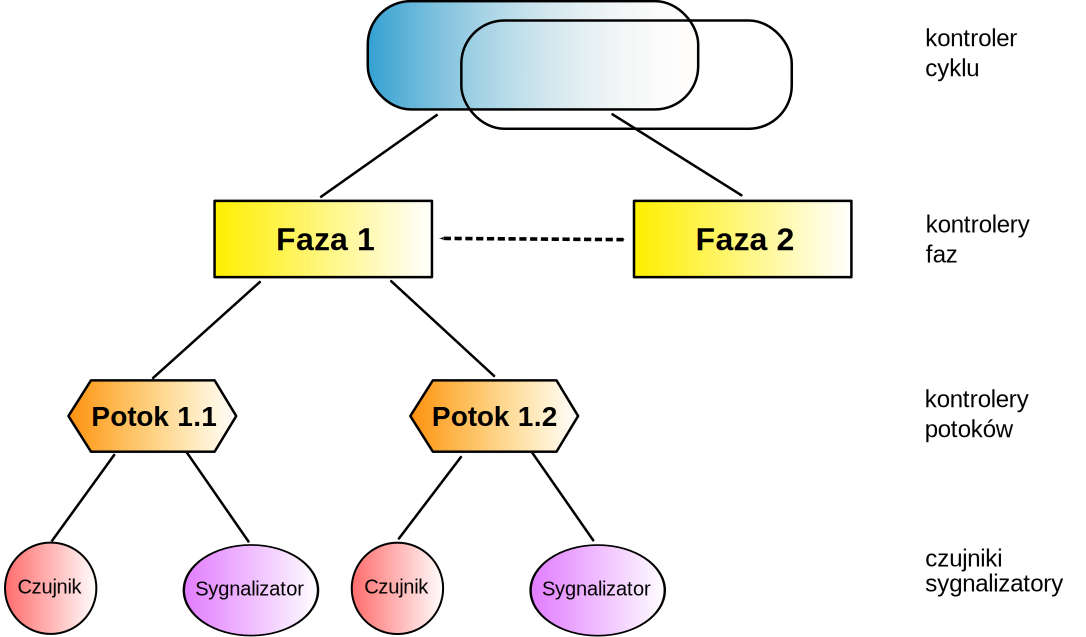
\includegraphics[width=0.9\textwidth]{img/models-hierarchy}
  \caption{Zależności między poszczególnymi komponentami modelu.}
  \label{img:hierarchy}
\end{figure}

\subsection{Czujniki i sygnalizatory}
\label{ss:models:models:dets}
Komponenty należące do najniższej warstwy systemu są prostymi
automatami czasowymi.
Sygnalizatory nie zawierają żadnych elementów sterowania, przyjmują
one jedynie polecenia zmiany sygnału (kanał \url{chg}) od właściwych
kontrolerów potoku (patrz \imgr{img:lights}).

\begin{figure}
  \centering
  \subfloat[Sygnalizator dla pojazdów]{
    \includegraphics[width=0.35\textwidth]{img/models-light-car}
  }
  \hspace{1cm}
  \subfloat[Sygnalizator dla pieszych]{
    \includegraphics[width=0.35\textwidth]{img/models-light-ped}
  }
  \caption{Automaty reprezentujące sygnalizatory}
  \label{img:lights}
\end{figure}

Czujniki zgłaszają zapotrzebowanie kontrolerom potoku poprzez
komunikat \url{act}. Czujniki dla pojazdów są w zasadzie automatami
jednostanowymi: w wierzchołku \url{Actuated} nie upływa czas. Rolę
zegara \url{zeno_t} omówiono w \ref{s:models:assumptions}, natomiast
zmiennej \url{service[id]} w \ref{s:models:opt}. Czujnik dla pieszych
ma natomiast dwa istotne stany, co modeluje zachowanie typowego
przycisku. Zwróćmy uwagę na fakt, że jest on jawnie resetowany
(\url{button_reset}).

\begin{figure}
  \centering
  \subfloat[Czujnik dla pojazdów]{
    \includegraphics[width=0.4\textwidth]{img/models-detector-car}
  }
  \hspace{1cm}
  \subfloat[Czujnik dla pieszych]{
    \includegraphics[width=0.4\textwidth]{img/models-detector-ped}
  }
  \caption{Automaty reprezentujące czujniki}
  \label{img:detectors}
\end{figure}

\subsection{Kontroler potoku}
Kontroler potoku zarządza pracą pojedynczego sygnalizatora poprzez
decydowanie o długości wyświetlanych sygnałów (w ramach wyznaczonych
przez odpowiedni kontroler fazy). Odbiera on również zgłoszenia od
odpowiedniego czujnika.

Poniżej znajduje się opis modelu kontrolera w pełni wzbudzanego potoku
dla pojazdów.
\paragraph{Struktura} Funkcję kontrolera potoku pełni jeden automat o
następujących parametrach:
\begin{itemize}
  \item \url{id} -- identyfikator potoku;
  \item \url{pid} -- identyfikator fazy, w skład której wchodzi dany potok;
  \item \url{RED_AMBER}, \url{INIT_GREEN}, \url{AMBER},
  \url{RED_CLEAR}, \url{GAP} -- parametry decydujące o długości
  poszczególnych sygnałów.
\end{itemize}
Struktura kontrolera potoków jest ściśle związana z nadawanymi
sygnałami (patrz \imgr{img:mvmt-ctrl}). Mamy zatem wierzchołek dla
każdego sygnału o stałej długości oraz zestaw wierzchołków dla
sygnałów o zmiennej długości. Wśród wierzchołków ,,zielonych''
wyróżniamy:
\begin{itemize}
  \item \texttt{InitialGreen} -- część początkowa,
  \item \texttt{ExtGreen} -- cześć rozszerzalna przed wykryciem luki,
  \item \texttt{GappedOut} -- cześć rozszerzalna po wykryciu luki,
  \item \texttt{Rest} -- stan spoczynku.
\end{itemize}
Natomiast sygnał czerwony związany jest z następującymi wierzchołkami:
\begin{itemize}
  \item \texttt{RedClear} -- okres czyszczenia
  \item \texttt{RedNoDemand} -- potok nieaktywny, brak zgłoszenia
  \item \texttt{RedWaiting} -- potok nieaktywny, przyjęto zgłoszenie
  od czujnika
\end{itemize}
Praca kontrolera potoku nadzorowana jest przez dwa zegary:
\begin{itemize}
  \item \texttt{fixed\_t} -- odpowiada za interwały (bądź ich części) o
  stałej długości,
  \item \texttt{gap\_t} -- odpowiada za długość części rozszerzalnej
  interwału zielonego; w momencie otrzymania zgłoszenia jest on
  resetowany, zatem osiągnięcie przezeń wartości równej wydłużeniu
  oznacza wykrycie luki.
\end{itemize}
\paragraph{Bazowy schemat funkcjonowania} Podstawowy cykl pracy
kontrolera potoku wzbudzanego przebiega następująco:
\begin{enumerate}
  \item Kontroler otrzymuje zgłoszenie od czujnika (\texttt{act?}) i przekazuje
  informację o zapotrzebowaniu do kontrolera fazy (\texttt{call!}).
  \item Kontroler odbiera polecenie startu od kontrolera fazy
  (\texttt{go?}) i przechodzi w stan aktywności.
  \item Kontroler zarządza nadanie sygnału czerwono-żółtego, a
  następnie części początkowej sygnału zielonego (\texttt{chg!})
  \item Po zakończeniu części początkowej, kontroler przechodzi do
  części rozszerzalnej; trwa ona aż do momentu, w którym zajdzie jeden
  z dwóch warunków:
  \begin{itemize}
    \item zostanie wykryta luka tj. zegar \url{gap_t} osiągnie wartość
    \url{GAP}; informacja o tym jest wysyłana do kontrolera fazy
    (\url{gapped_out!});
    \item kontroler fazy wyśle informację o osiągnięciu czasu
    maksymalnego (\texttt{maxed\_out?}).
  \end{itemize}
  \item Kontroler zarządza kolejno nadanie sygnału żółtego i
  czerwonego-czyszczącego (\texttt{chg!}), po czym zgłasza zakończenie pracy
  kontrolerowi fazy (\texttt{gone\_off!}).
\end{enumerate}

\begin{sidewaysfigure}
  \centering
  \includegraphics[width=0.9\textwidth]{img/models-mvmt}
  \caption{Model kontrolera potoku dla pojazdów.}
  \label{img:mvmt-ctrl}
\end{sidewaysfigure}

\subsection{Kontroler fazy}
Kontroler fazy zarządza funkcjonowaniem zależnych od siebie
kontrolerów potoków, wyznaczając początek i maksymalny czas ich pracy.

Poniżej opisano model wielopotokowego kontrolera fazy.
\paragraph{Struktura} Kontroler fazy składa się z dwóch
automatów. Pierwszy z nich odpowiada za logikę, zaś drugi wyłącznie za
odmierzanie czasu maksymalnego. Główny automat komunikuje się z
automatem-zegarem wysyłając mu polecenia \url{timer_on} i
\url{timer_off}. Podział komponentu na dwie części pozwolił na
zmniejszenie liczby wierzchołków i ogólne uproszczenie jego konstrukcji.

Główna część kontrolera fazy jest automatem o następujących
parametrach:
\begin{itemize}
  \item \url{id} -- identyfikator fazy;
  \item \url{m1}, \url{m2}, ... -- identyfikatory składających się na
  nią potoków;
  \item \url{MAX} -- maksymalny zielony.
\end{itemize}
Jak w typowym automacie sterującym, większość jej wierzchołków jest
oznaczonych jako przymusowe; do pozostałych należą:
\begin{itemize}
  \item \url{Inactive} -- faza nieaktywna, brak zapotrzebowania;
  \item \url{InactiveWaiting} -- faza nieaktywna, oczekiwanie na
  polecenie startu;
  \item \url{Active} -- faza aktywna;
  \item \url{GoingOff} -- oczekiwanie na potwierdzenia zakończenia
  pracy przez potoki.
\end{itemize}
W jego skład wchodzą także poniższe zmienne:
\begin{itemize}
  \item \url{mvmts_on : int} -- liczba aktywnych potoków,
  \item \url{mvmts_not_out : int} -- liczba potoków, w których nie wykryto luki,
  \item \url{call_arr[mvmts] : bool} -- dane o zapotrzebowaniu,
  \item \url{held[mvmts] : bool} -- dane o podtrzymanych sygnałach,
  \item \url{timer_set : bool} -- informacja o aktywności zegara czasu
  maksymalnego
\end{itemize}

\paragraph{Bazowy schemat działania} Podstawowy cykl funkcjonowania
kontrolera przebiega następująco:
\begin{enumerate}
  \item Kontroler przyjmuje zgłoszenie od jednego z potoków (\url{call?}) i
  przekazuje informacje o zgłoszeniu przeciwnym kontrolerowi aktywnej
  fazy lub kontrolerowi cyklu w przypadku spoczynku w czerwonym (\url{opp!}).
  \item Kontroler dostaje polecenie startu od kontrolera cyklu
  (\url{start?}), przekazuje je tym kontrolerom potoków, które
  zgłosiły zapotrzebowanie (\url{go!}). Jeśli już w tym momencie jest
  zapotrzebowanie przeciwne, uruchamiany jest zegar czasu
  maksymalnego.
  \item Kontroler przechodzi w główny stan cyklu, w którym obsługuje
  następujące komunikaty od kontrolerów potoków:
  \begin{itemize}
    \item informacje o wykryciu luki (\url{gapped_out?}),
    \item informacje o zakończeniu pracy (\url{gone_off?}),
    \item zgłoszenia późne (\url{call?}).
  \end{itemize}
  Konkretne działanie podejmowane w każdym z powyższych przypadków
  zależą od wybranych opcji. Jeśli zgłoszenie przeciwne
  (\url{opp?}) nie zostało obsłużone wcześniej, to może zostać
  obsłużone w tym stanie tj. uruchomiony będzie zegar czasu
  maksymalnego.
  \item Aktywność fazy może zostać zakończona z dwóch powodów:
  \begin{itemize}
    \item każdy z kontrolerów przekazał informację o wykryciu luki
    (\url{mvmts_not_out == 0}) bądź o zakończeniu pracy
    (\url{mvmts_on == 0}),
    \item osiągnięty został czas maksymalny.
  \end{itemize}
  W chwili wystąpienia jednego z tych warunków kontroler przechodzi w
  ostatni etap swojej pracy. Wysyła wszystkim potokom, które nadal
  wyświetlają sygnał zielony (w szczególności -- podtrzymanym)
  polecenie zakończenia pracy (\url{go_off!}) i czeka na otrzymanie
  potwierdzenie jego wykonania (\url{gone_off?}). Następnie przechodzi
  w jeden ze stanów nieaktywności, informując o tym kontroler cyklu
  (\url{finished!}).
\end{enumerate}

\begin{sidewaysfigure}
  \centering
  \includegraphics[width=1.1\textwidth]{img/models-phasectrl}
  \caption{Model kontrolera fazy (składającej się z dwóch w pełni wzbudzanych potoków dla pojazdów).}
  \label{img:phase-ctrl}
\end{sidewaysfigure}

\subsection{Kontroler cyklu}
\label{ss:models:models:ring}
Kontroler cyklu jest najprostszym z przedstawionych elementów
sterowania sygnalizacją (patrz \imgr{img:ring-ctrl}). Jego jedynym
parametrem jest \url{rest_ph} -- numer fazy spoczynkowej.

Kontroler cyklu uruchamia pierwszą kolejności fazę, na którą
jest zapotrzebowanie (\url{start!}), następnie zaś czeka na
potwierdzenie zakończenia jej aktywności (\url{finished?}). Gdy nie ma
zapotrzebowania na żadną fazę kontroler przechodzi w stan spoczynku
bądź uruchamia fazę spoczynkową.

\begin{figure}
  \centering
  \includegraphics[width=0.6\textwidth]{img/models-ring}
  \caption{Model kontrolera cyklu}
  \label{img:ring-ctrl}
\end{figure}

\subsection{Podsumowanie}
\label{ss:models:models:summary}
% \todo{
% mamy sobie hierarchię, każdy rządzi kimś i jest rządzony przez kogoś

% kluczową rolę w sterowaniu odgrywają kontrolery potoku i fazy,
% one zarządzają czasem

% może i jest dużo komunikatów, ale pozwala to uniezależnić od siebie 
% }

Tabela \ref{tab:models:channels} podsumowuje najważniejsze kanały
komunikacyjne modelu, natomiast \imgr{img:models:msc} przedstawia
podstawowy schemat komunikacji.

\renewcommand{\arraystretch}{1.4}
\begin{table}
  \centering
  \begin{tabular}{>{\scshape}r|p{0.35\textwidth}|>{\ttfamily}p{0.25\textwidth}}
    \firsthline\firsthline
    \textbf{Komponenty} & \textbf{Komunikat} & \textnormal{\bfseries Nazwa kanału} \\ \hline
    Czujnik \rarr\ Potok & zgłoszenie & act[mvmt\_id] \\ \hline
    Potok \rarr\ Sygnalizator & polecenie zmiany sygnału & chg[mvmt\_id]
    \\ \hline
    Potok \rarr\ Faza & zgłoszenie zapotrzebowania & call[phase\_id] \\
                      & informacja o wykryciu luki & gapped\_out[phase\_id] \\
                      & potwierdzenie zakończenia aktywności & gone\_off[phase\_id]
    \\ \hline
    Faza \rarr\ Potok & polecenie startu & go[mvmt\_id] \\
                      & polecenie zakończenia & go\_off[mvmt\_id] \\
                      & osiągnięcie czasu maksymalnego & maxed\_out[phase\_id]
    \\ \hline
    Faza \rarr\ Faza & zgłoszenie przeciwne & opp
    \\ \hline
    Cykl \rarr\ Faza & polecenie startu & start \\ \hline
    Faza \rarr\ Cykl & potwierdzenie zakończenia aktywności & finished \\
    \hline\hline
  \end{tabular}
  \caption{Komunikacja między komponentami.}
  \label{tab:models:channels}
\end{table}

\begin{figure}
  \centering
  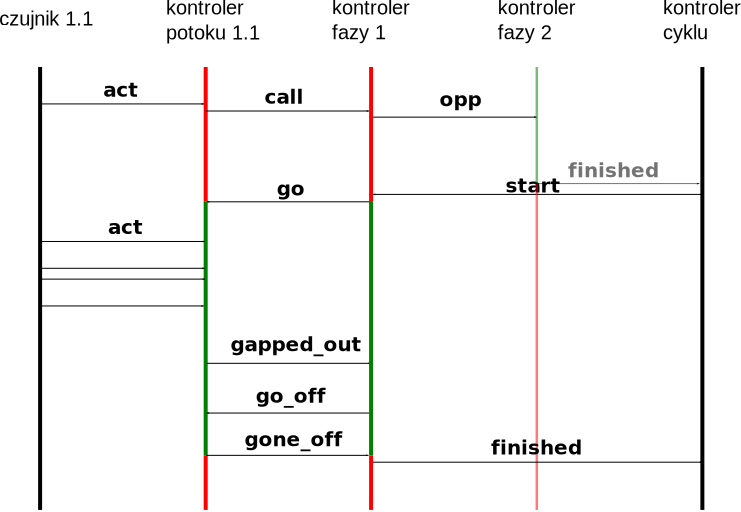
\includegraphics[width=0.8\textwidth]{img/models-msc}
  \caption{Podstawowy schemat komunikacji pomiędzy procesami.}
  \caption*{Schemat przedstawia komunikację w jednym cyklu aktywności
    fazy. Dla uproszczenia pominięto komunikację kontrolera potoku z
    sygnalizatorem oraz komunikację między komponentami fazy 2.}
  \label{img:models:msc}
\end{figure}


\section{Decyzje projektowe}
\label{s:models:project}

Sposób konstrukcji modelu wynika nie tylko z samej istoty postawionego
zadania, lecz także z pewnych ogólnych zasad inżynierii
oprogramowania. Podjęte decyzje projektowe wynikają z dążenia do
osiągnięcia następujących własności modelu:
\begin{enumerate}
  \item możliwie dokładne odzwierciedlenie funkcjonowania docelowego systemu,
  \item konfigurowalność,
  \item utrzymywalność i czytelność,
  \item weryfikowalność,
\end{enumerate}
Konstrukcja automatów przebiegała w dwóch etapach. W pierwszym,
kierując się głównie założeniami 1-3, przygotowano ogólną strukturę
modelu oraz wstępne wersje poszczególnych automatów. Następnie, o ile
dostępne zasoby nie pozwalały na weryfikację oczekiwanych własności,
automaty były optymalizowane.

\subsection{Wstępna konstrukcja modelu}

W pierwszym etapie pracy system został podzielony na komponenty,
określono ich odpowiedzialności oraz interfejsy, przy pomocy których
komunikują się z pozostałymi. Kierowano się przede wszystkim ogólnie
znanymi zasadami prawidłowego projektowania oprogramowania takimi jak
ukrywanie wewnętrznej implementacji komponentów czy unikanie
powtarzania się podobnych elementów struktury. Już na tym etapie
należało zadbać o wydajność weryfikacji, co polegało m.in. na
minimalizacji liczby zmiennych (przede wszystkim -- zegarowych) oraz
oznaczaniu wierzchołków jako przymusowe.

\subsection{Optymalizacja modeli}
\label{s:models:opt}

Celem optymalizacji modelu jest redukcja zasobów, tj. pamięci
operacyjnej i czasu procesora, potrzebnych do zweryfikowania pewnych
jego własności. Poniżej przedstawiono najważniejsze z zastosowanych metod.

\paragraph{Minimalizacja liczby przeplotów} Podstawowym środkiem
służącym optymalizacji modelu jest minimalizacja liczby możliwych
przeplotów i -- co za tym idzie -- zmniejszenie przestrzeni stanów
przeszukiwanej w czasie weryfikacji\footnote{Znaczenie ograniczania
  liczby przeplotów jest tym większe, że w \upp-u nie zaimplementowano
  redukcji częściowo-porządkowych.}. Najprostszą metodą osiągnięcia
tego celu jest wspomniane wyżej oznaczanie wierzchołków jako przymusowe.
Innym sposobem jest uniemożliwienie wykonania tranzycji, które nie
mają znaczenia z punktu widzenia funkcjonowania docelowego
systemu. Przykładem tego działania było pominięcie nieistotnych,
tj. niemających wpływu na pracę kontrolera, wzbudzeń czujnika. Należą
do nich m.in. wzbudzenia w początkowej części interwału zielonego lub
wzbudzenia dla nieaktywnego potoku, gdy już wcześniej zostało
zgłoszone zapotrzebowanie. Aby je wyeliminować, dla każdego potoku
wprowadzono zmienną boolowską \url{service}. Kontroler ustawia
jej wartość na prawdziwą, gdy wzbudzenia czujnika są istotne oraz
fałszywą -- w przeciwnym przypadku. W automacie reprezentującym
czujnik dodano ograniczenie na krawędź, pozwalające mu przejść w stan
wzbudzenia wyłącznie, gdy \url{service} ma wartość prawdziwą.

\paragraph{Redukcja zmiennych aktywnych} Kolejną ważną metodą
optymalizacji modeli jest \emph{redukcja zmiennych aktywnych}.
Chociaż wartości wszystkich zmiennych są stale utrzymywane w modelu,
czasem zachodzi sytuacja, w której w pewnych stanach wartość
niektórych z nich nie ma znaczenia: dwa stany różniące się wyłącznie
takimi zmiennymi można uznać za identyczne. Zresetowanie wartości tych
zmiennych utożsami zatem te stany, co zmniejszy rozmiar przeszukiwanej
przy weryfikacji przestrzeni.

Powyższe rozważania formalizuje następująca definicja: zmienną $v$
nazywamy \emph{nieaktywną} w wierzchołku $l$, gdy na wszystkich
ścieżkach zaczynających się w $l$, $v$ zostanie zresetowana zanim
zostanie odczytana. Jeśli zmienna $v$ jest nieaktywna w wierzchołku
$l$ należy zresetować jej wartość na wszystkich krawędziach
prowadzących do $l$. Wyjątkiem jest sytuacja, w której $v$ jest
nieaktywna już we wszystkich wierzchołkach, z których prowadzą
krawędzie do $l$. Wtedy jej wartość została zresetowana już wcześniej
i nie ma potrzeby powtarzania tej operacji.

\upp\ przeprowadza analizę aktywności zmiennych zegarowych w trakcie
weryfikacji, zatem zasadniczo nie ma potrzeby ręcznego resetowania
nieaktywnych zmiennych. Niestety automatyczna analiza często zawodzi w
przypadku, gdy mamy do czynienia z tablicami zegarów. Dlatego też w
automacie odmierzającym czas maksymalny, wprowadzono jawne resetowanie
zegarów (patrz \imgr{img:models-active-reduction}).

\begin{figure}
  \centering
  \subfloat[Zegar czasu maksymalnego bez jawnej redukcji nieaktywnej zmiennej.] {
    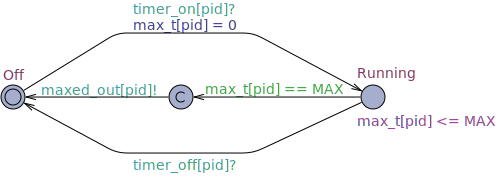
\includegraphics[width=0.45\textwidth]{img/models-maxtimer-noactred}
  }\hfill
  \subfloat[Zegar czasu maksymalnego z jawną redukcją nieaktywnej zmiennej.] {
    \includegraphics[width=0.45\textwidth]{img/models-maxtimer}
  }
  \caption{Redukcja zmiennych aktywnych}
  \label{img:models-active-reduction}
\end{figure}

\paragraph{Abstrakcja} Zaproponowane wyżej metody optymalizacji modeli
nie powodują zmniejszenia dokładności, z jaką reprezentowany jest
docelowy system. Często okazują się one jednak niewystarczające, aby
móc dowieść jego pożądanych własności. Należy wtedy uprościć model,
rezygnując z reprezentowania tych cech systemu, które są nieistotne
dla danej własności.

Przykładem takiego uproszczenia jest pominięcie nadawania sygnałów
czerwono-żółtego i żółtego. Metoda ta została zastosowana przy
weryfikacji najbardziej skomplikowanych systemów.
% Jako, że są one
% zarządzane wyłącznie przez kontroler potoku, taka abstrakcja nie
% powinna mieć na wpływu własności dotyczące poprawnej współpracy
% komponentów systemu.

\chapter{Eksperymenty}


Mam następujący pomysł na ten rozdział:
\begin{enumerate}
  \item W pierwszej części zweryfikować bazowy zestaw własności dla
  dwóch w miarę prostych modeli. Na ich podstawie poruszyć kwestie
  takie jak:
  \begin{itemize}
    \item problem z weryfikacją pełnej żywotności (trwa bardzo długo)
    i jego rozwiązanie: weryfikacja żywotności ograniczonej (nie dość,
    że jest ona dużo istotniejsza, to jeszcze prościej ją sprawdzić --
    \emph{de facto} jest własnością bezpieczeństwa
    \item praktycznie wszystkie własności bezpieczeństwa da się
    zweryfikować, przybliżając strefy z góry (przez otoczkę wypukłą);
    pozwala to na weryfikację tych własności nawet w bardzo dużych
    modelach
  \end{itemize}
  \item W drugiej części nieco rozwinąć zestaw weryfikowanych
  wartości; kładąc nieco więcej nacisku na weryfikację cech
  ilościowych.
  \item W trzeciej części pokazać ciekawe -- z punktu widzenia ich
  weryfikacji -- własności modeli.
  \begin{itemize}
    \item Przede wszystkim pokazać zależność rozmiaru przestrzeni
    stanów rozmiaru modelu i jego parametrów. Głównym bohaterem będzie
    tu z pewnością \url{A[] not deadlock}, gdyż nie daje się ona
    szybko zweryfikować przy pomocy otoczki wypukłej.
    \item Mógłbym też pokazać jak na czas weryfikacji wpływają
    optymalizacje opisane w \ref{s:models:opt}.
  \end{itemize}
\end{enumerate}

% \section{Podstawowe własności}

% \begin{enumerate}
%   \item \url{A[] ((MvC00.InitialGreen || MvC00.ExtGreen || MvC00.GappedOut || MvC00.Rest) imply L00.Green)}
%   \item \url{A[] ((MvC00.RedClear || MvC00.RedNoDemand || MvC00.RedWaiting) imply L00.Red)}
%   \item \url{A[] (MvC00.RedAmber imply L00.RedAmber)}
%   \item \url{A[] (MvC00.Amber imply L00.Amber)}
%   \item \url{A[] (PC0.Inactive imply (MvC00.RedNoDemand || MvC00.RedGotCall || MvC00.RedWaiting))}
%   \item \url{A[] (PC0.InactiveWaiting imply (MvC00.RedNoDemand || MvC00.RedGotCall || MvC00.RedWaiting))}
%   \item \url{A[] (PC0.Active + PC1.Active <= 1)}
%   \item \url{A[] not deadlock}
%   \item \url{Det00.Actuated --> L00.Green}
%   \item \url{!service[M00] --> L00.Green}
% \end{enumerate}

% \begin{table}
%   \centering
%   \begin{tabular}{|r|| l|l|l || l|l|l || l|l|l|}
%     \hline
%     Nr & \multicolumn{3}{c||}{Najmniejsze} & \multicolumn{3}{c||}{DBM} & \multicolumn{3}{c|}{Otoczka} \\ \hline
%        & Wynik & Czas[s] & L.~st. & Wynik & Czas & L.~st. & Wynik & Czas & L.~st \\
%     1. & TAK & $<1$ & 10068 & TAK & $<1$ & 10068 & TAK & $<1$ & 6391\\
%     2. & TAK & $<1$ & 10068 & TAK & $<1$ & 10068 & TAK & $<1$ & 6391\\
%     3. & TAK & $<1$ & 10068 & TAK & $<1$ & 10068 & TAK & $<1$ & 6391\\
%     4. & TAK & $<1$ & 10068 & TAK & $<1$ & 10068 & TAK & $<1$ & 6391\\
%     5. & TAK & $<1$ & 10068 & TAK & $<1$ & 10068 & TAK & $<1$ & 6391\\
%     6. & TAK & $<1$ & 10068 & TAK & $<1$ & 10068 & TAK & $<1$ & 6391\\
%     7. & TAK & $<1$ & 10068 & TAK & $<1$ & 10068 & TAK & $<1$ & 6391\\
%     8. & TAK & 12   & 37720 & TAK & 11 & 37720 &  ? & $<1$ & 15994\\
%     9. & TAK & 25   & -     & TAK & 22 & - & ? & $<1$ & -\\
%     10.& TAK & 36   & -     & TAK & 32 & -&  ? & $<1$ & -\\
%     \hline
%   \end{tabular}
%   \caption{Weryfikacja podstawowych własności dla modelu XXX}
%   \label{tab:ver-sr-22}
% \end{table}

\addcontentsline{toc}{chapter}{Bibliografia}
\bibliography{bib.bib}{}
\bibliographystyle{plalpha}
\end{document}

%%% Local Variables:
%%% mode: latex
%%% TeX-master:
%%% coding: utf-8
%%% eval: (auto-fill-mode 1)
%%% End:

% LocalWords:  stałoczasowa jednopotokowych wielopotokowej Alura Dilla TCTL
% LocalWords:  Henzingera stałoczasowym stałoczasowych kompozycjonalny
% LocalWords:  boolowskiego konfigurowalność boolowską utrzymywalność
% LocalWords:  wielopotokowych stałoczasowego jednostanowymi zenonowskie
% LocalWords:  niezenonowski Zenonowskość zenonowskimi wysokopoziomowość
% LocalWords:  wyspecyfikować niskopoziomowości rozgłoszeniowy zenonowski
